\documentclass{beamer}
\usepackage[latin1]{inputenc}

\usepackage[noend]{algpseudocode}
\usepackage[ruled]{algorithm}
\usepackage{url}
\usepackage{framed}
\usepackage{amsfonts,amsmath,amsthm}
\usepackage{graphicx}
\usepackage{url}
\usepackage{color}

\title{}
\author{}
\institute{}
\date{}

\AtBeginSection[]
{
  \begin{frame}<beamer>
    \frametitle{Outline}
    \tableofcontents[currentsection]
  \end{frame}
}


\begin{document}

% \begin{frame}
% \titlepage
% \end{frame}

\begin{frame}{Upper Bounds on Value of Information}
\end{frame}

\begin{frame}{Sampling in Trees}
\begin{itemize}
\item Hybrid sampling scheme:
\begin{enumerate}
\item At the {\it root node}: sample based on the VOI estimate.
\item At {\it non-root nodes}: sample using UCT.
\end{enumerate}
\item Stopping Criterion
\end{itemize}
\end{frame}

\begin{frame}{Sample Redistribution}
\begin{itemize}
\item<+-> The VOI estimate assumes that the information is {\bf discarded}
  between states.
\item<+-> MCTS {\bf re-uses rollouts} generated at earlier search states.
\vspace{\baselineskip}
\item<+-> Either incorporate `future' influence into the VOI estimate
  ({\it non-trivial!}).
\item<+-> Or behave myopically w.r.t. search tree depth:
\begin{enumerate}
\item Estimate VOI as though the information is discarded.
\item Stop early if the VOI is below a certain threshold.
\item Save the unused sample budget for search in future states.
\end{enumerate}
\item<+-> The cost $c$ of a sample  is\\\hspace{1em} the VOI of increasing a
  future budget by one sample.
\end{itemize}
\end{frame}

\begin{frame}{Playing Go Against UCT:\\\hspace{2em}Tuning the Sample Cost}
\begin{figure}[h]
  \centering
  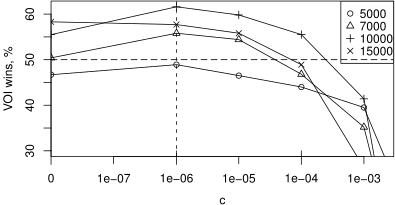
\includegraphics[scale=0.65]{uctvoi.pdf}
\end{figure}
Best results for sample cost $c\approx 10^{-6}$:\\\hspace{2em}winning rate of {\bf
  64\%} for 10000 samples per ply.
\end{frame}

\begin{frame}{Playing Go Against UCT:
    \\\hspace{1em} Winning Rate vs. Number of Samples per Ply}

Sample cost $c$ fixed at $10^{-6}$:
\begin{figure}
  \centering
  \includegraphics[scale=0.65]{voi-wins.pdf}
\end{figure}
Best results for {\it intermediate} $N_{samples}$:
\begin{itemize}
\item When $N_{samples}$ is too low, poor moves are selected.
\item When $N_{samples}$ is too high, the VOI of further sampling
  is low.
\end{itemize}
\end{frame}

\end{document}
